\section{Theorie}
\label{sec:Theorie}
Unter einer Linse wird allgemein ein Objekt verstanden, welches meist optisch dichter als das es umgebende Medium ist.
Beim Übergang eines Lichtstrahls zwischen zwei Medien unterschiedlicher optischer Dichte treten nach dem Brechungsgesetz Brechungseffekte auf.
In der Optik wird zwichen verschiedenen Linsen unterschieden.
Bei dünnen Linsen lässt sich die Brechung auf die Mittelebene der Linse reduzieren.
Eine Sammellinse wird zum Linsenrand hin dünner, sie bündelt parallel einfallendes Licht in dem sogennanten Brennpunkt. Entsprechend sind die Brennweite $f$ und die Bildweite $b$ positiv gezählt und es ensteht, wie in Abbildung \ref{fig:sammelli} ein reeles Bild.
Unter dem Begriff reeles Bild wird ein Bild verstanden, von dem reale Strahlen ausgehen. Im Gegensatz dazu ist ein imaginäres Bild ein Bild von dem keine reale Strahlen ausgehen so suggeriert ein Blick in den Spiegel zum Beispiel, dass sich Objekte ebenso weit hinter dem Spiegel stehen, wie sie im Realen vor dem Spiegel sind.
%Jaaa nice wrapfigures mal wieder!!!11
\begin{wrapfigure}{r}{0.45\textwidth}
  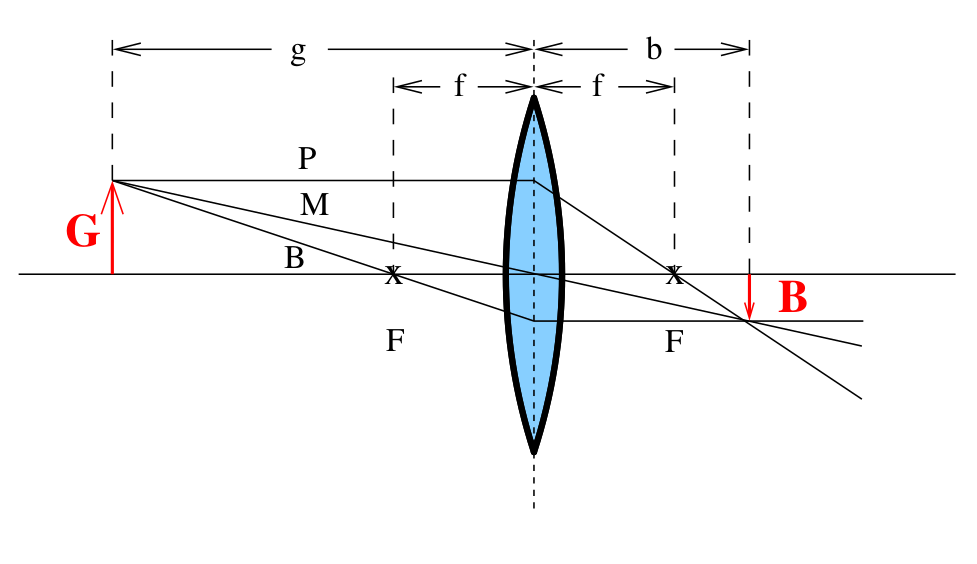
\includegraphics[width=\linewidth]{Bilder/sammellinse.png}
  \caption{Schematischer Strahlverlauf bei einer Sammellinse \cite{Anleitung}}
  \label{fig:sammelli}
\end{wrapfigure}
Bei einer Streulinse hingegen werden einfallende Strahlen nicht fokussiert, sondern vom Zentrum weggebrochen. Die gedachte Verlängerung der Strahlen auf der Seite der einfallenden Strahlen führt schließlich zum virtuellen Bild. Daher sind Bildweite und Brennweite auch negativ.
Im Gegensatz zu dünnen Linsen ist die Reduktion der Brechung nur auf die Mittelebene bei dicken Linsen nicht möglich. Stattdessen werden zwei Hauptebenen eingeführt.
Es wird vereinfachend angenommen, dass zwischen diesen beiden Hauptebenen der Linse alle Strahlen parallel laufen.

\begin{wrapfigure}{r}{0.45\textwidth}
  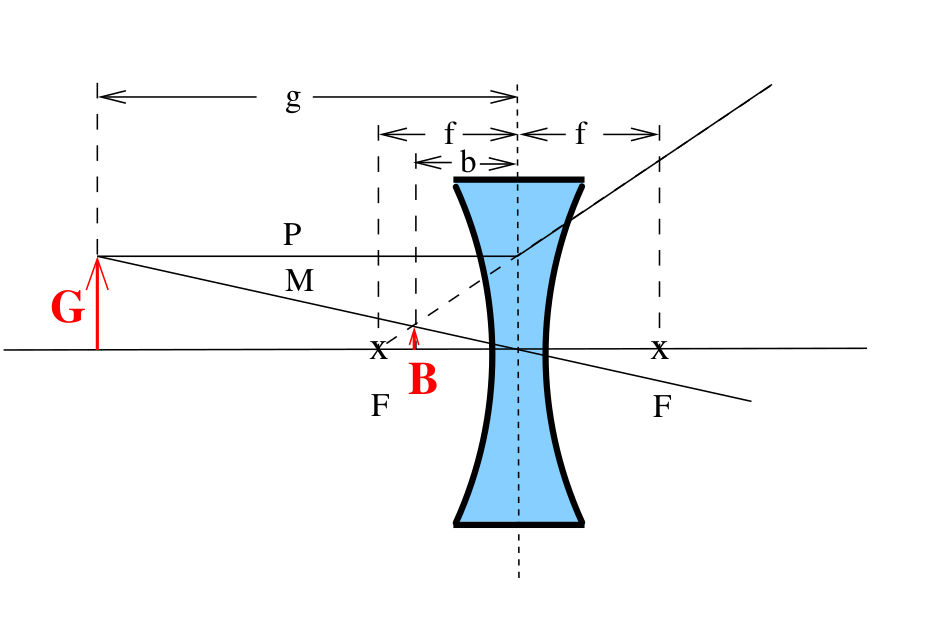
\includegraphics[width=\linewidth]{Bilder/streulinse.png}
  \caption{Schematischer Strahlverlauf bei einer Streulinse \cite{Anleitung}}
  \label{fig:streuli}
\end{wrapfigure}
\blindtext
\begin{wrapfigure}{r}{0.45\textwidth}
  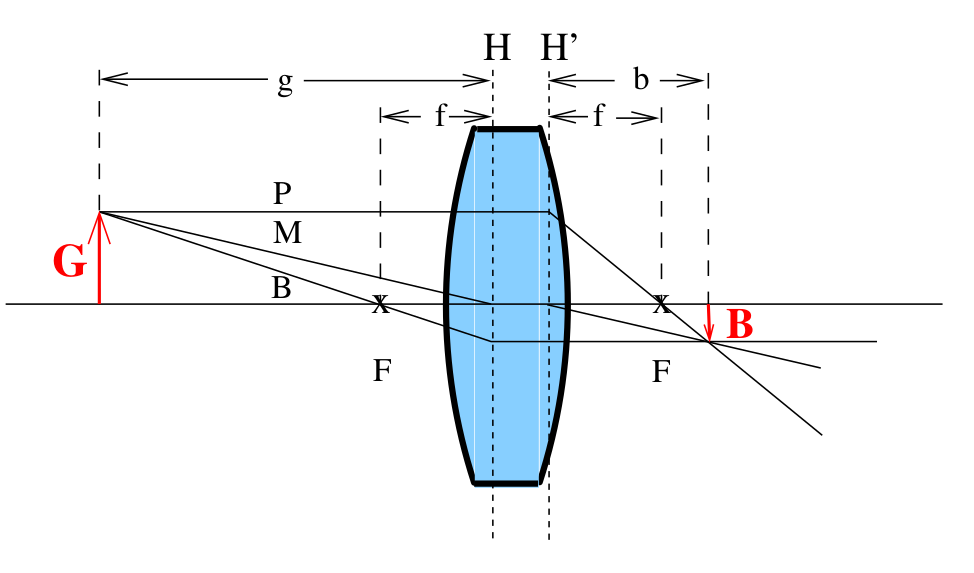
\includegraphics[width=\linewidth]{Bilder/fettelinse.png}
  \caption{Schematischer Strahlverlauf bei einer dicken Sammellinse \cite{Anleitung}}
  \label{fig:diefette}
\end{wrapfigure}
